% Chapter Template

\chapter{Pilot study} % Main chapter title

\label{Pilotstudy} % Change X to a consecutive number; for referencing this chapter elsewhere, use \ref{ChapterX}

%----------------------------------------------------------------------------------------
%	SECTION 1
%----------------------------------------------------------------------------------------
The goal of this pilot study is to test if the layout will be able to give any significant results. Further, the pilot study will also test if the tasks in the study can answer our goal questions. The pilot study will also give a clearer indication of the potential limitations this study will have.
\section{Method}
The pilot study was done by showing the testing users the developed sketch prototype. Using this sketch prototype the tester sat next to the user and asked them to perform the tasks written down on a piece of paper (In Chinese for the Chinese users and in English for the Western users). First, the participants got a minute to look around the page to get a quick feel for the layout of the site. Then a question was shown to the user and a timer was started simultaneously. When the test subject found the requested image or text, they indicated that they had found the information and the timer was then stopped. If a user could not find a certain piece of information, they were allowed to skip that question. This was repeated until all the tasks were fulfilled.

\section{Results}
The users where asked to perform the following tasks:
\\\\
\textbf{English BBC Questions:}
\begin{enumerate}
	\item Click the news about ivory stabbing
	
	\item Click on the Korean men beauty revolution
	
	\item Click on the news about the freed samung heir
	
	\item Click on the news about Zuma refusing to step down.
	
	\item Click on the news that has to do with a angry sports coach.
	
	\item Click on the long read article about the catholic priest father
	
	\item Click on the video about cooking with strangers
	
	\item Click on the video that has to do with Indonesia

	\item Via the top menu go to the new phones site
	
	\item Via the top menu go to US politics
	
	\item Via the top menu go to news about the stock market
	
\end{enumerate}

\textbf{English QQ Questions}:
\begin{enumerate}

	
	\item Click on the following news: One hundred Hongkong staff more than half hiding in the United States and Canada
	
	\item Click on the following news: Fishermen are no longer allowed to bring their own baits.
	
	\item Click on the following news: Russian fighter pilots last words before blowing himself up with a grenade “For my brothers"
		
	\item Click the following news: True beauty don’t fear wrinkles
		
	\item Click on the video with a Chimpanzee
	
	\item Click on the video below: Premier League - Liverpool 2-2
		
	\item Click on the skyscraper picture
		
	\item Click on the news below: Dow plunge near 700 on Friday what trigged it?
		
	\item Choose from the following menu items: News
		
	\item Choose from the following menu items: Health
		
	\item Choose from the following menu items: Sports
	
	\item Choose from the following menu items: Digital
\end{enumerate}
The BBC pilot study resulted in the following results (see fig \ref{fig:pilot_study_bbc}): 
\begin{figure}[h]
	\centering
	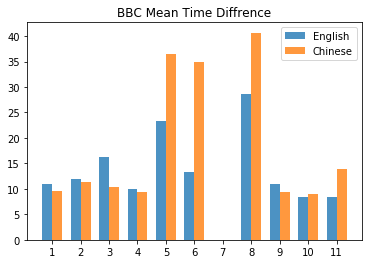
\includegraphics[width=60mm]{Images/pilot_study_bbc_mean_time}
	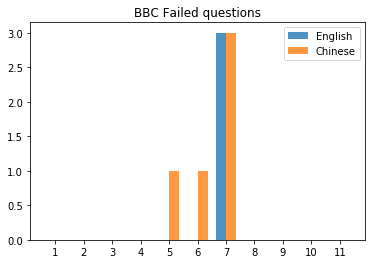
\includegraphics[width=60mm]{Images/pilot_study_bbc_failed}
	\decoRule
		\caption[BBC pilot study results]{Results from the pilot study for the BBC inspired news prototype.}
	\label{fig:pilot_study_bbc}
\end{figure}
\newpage
The QQ pilot study resulted in the following mean results (see fig \ref{fig:pilot_study_qq}):
\begin{figure}[h]
	\centering
	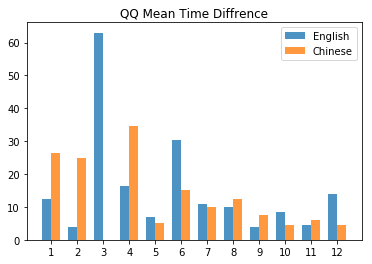
\includegraphics[width=60mm]{Images/pilot_study_qq_mean_time}
	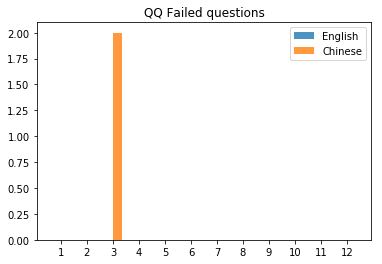
\includegraphics[width=60mm]{Images/pilot_study_qq_failed}
	\decoRule
	\caption[QQ pilot study results]{Results from the pilot study for the QQ inspired news prototype.}
	\label{fig:pilot_study_qq}
\end{figure}

\section{Discussion}
This pilot study revealed a lot of relevant issues. One main problem was that some of the news was repeated in several places of the site. This made some tasks irrelevant since the news could be located at several different locations. Additionally, some questions were badly translated as well. For example, the question of the sports coach seemed to confuse many of the Chinese users. Also, the questions regarding finding images on the qq site did not provide with any meaningful result since QQ has very few pictures and therefore they did not check how well the user performed in information-dense sites. Another thing that was noticed during the test was how the order of the tasks affected task success. All the users quickly found news closely located to the previous task. This needs to be kept in mind when designing the next set of questions.
\\\\
We can see the measurements from the study in \ref{fig:pilot_study_bbc} and \ref{fig:pilot_study_qq}. Since the goal of the pilot study was to try out if the concept for the real study works, we did not have enough participants for this data to have any statistical significance. As mentioned above, the goal of the study was to find problems with the questions, translation and user-experience. According to Norman(year) we only need about 5 participants to find the majority of user experience problems. However, if we want this survey to be statistically significant when actually measuring time differences we would need a larger amount of users.


\section{Conclusion}
Many questions will be changed to obtain better results for the projects, also both the sites will have the same structure for its tasks. Both sites will have 13 tasks to perform. Four of the tasks will be about the menu-bar, four of the tasks will be about finding precisely described news titles, one task will be about following the page on social media and lastly, 4 of the tasks will be about finding more general described news. About half of the tasks will be in the F-shaped pattern view sight. The other half of the questions will be located on the right-hand and central side of the website. Finally, the sites will be designed so the ad content of both sites will be adjusted to the language of the site (i.e BBC in Chinese will have Chinese ads and vice versa). 
\\\\
Some functionality will be added to the prototype such as giving feedback and also following on social media. This will be done according to standards as can be seen in \ref{Chapter4}. A menu with the option to give feedback and follow on social media will be added to the right hand side on the Chinese pages respectively on the bottom of the page for the western site.

\subsection{BBC Questions}
The new questions selected for bbc are the following:
\begin{enumerate}
\item In the menu Click on: Phones
\item In the menu Click on: Music
\item In the menu Click on: USA Politics
\item In the menu Click on: Africa
\item Click on the following news segment: Breastfeeding mother sells milk on street
\item Click on the following news segment: Samsung heir freed from S Korea jail
\item Click on the following news segment: From a broken neck to a Rhodes Scholarship at Oxford
\item Click on the following news segment: How Ikea has changed the way we shop
\item Click on the news about a challenge to become vegan
\item Click on the news that has to do with Indonesia
\item Click on the news article about the president refusing to step down
\item Click on the news about the killed NFL player
\item Follow the page on Twitter
\end{enumerate}
\subsection{QQ Questions}
The questions selected for qq are the following:
\begin{enumerate}
	\item In the menu bar select: Military
	\item In the menu bar select: Furniture
	\item In the menu bar select: Celebrity
	\item In the menu bar select: Culture
	\item Click on the following news: Dow plunge nearly 700 points on Friday what triggerd it?
	\item Click on the following news segment: True beauty don’t fear wrinkles
	\item Click on the following news segment: One hundred Hongkong staff more than half hiding in the United States and Canada
	\item Click on the following news segment: 7-year-old boy earns hundreds of thousands determins to financialy support parents
	\item Follow the page on Twitter
	\item Select the news about Engineers testing fruit
	\item Select the news article with a picture in the Real Estate category
	\item Select the picture with a burning airplane
	\item Select the news about gold coins found in a shipwreck
\end{enumerate}
